% !TeX root = ../main.tex

\chapter{引言}
\label{cha:intro}
\section{研究背景与意义}
%%% 叙事结构
% 视觉语言
% 预训练-微调
% 联合微调
% 联合预训练->language supervised
%%%

%%% 视觉-语言的生物学、认知学、演化学性质
% 整体:视觉和语言是人类重要的信息获取、交换方式(扯一些高级东西,大脑皮层的处理,生物学的东西),讲一下视觉与语言的结构共享,互相影响等等(可以从《我们赖以生存的意义》里找些论据)。需要强调视觉能力受语言能力的影响。
% 参考:视觉信息在人类所接收到的信息中占据了主导地位,它是我们感知周围环境、定位目标和进行认知识别等一系列复杂活动的基础。为了实现这些高度复杂的功能,人类视觉皮层经过数百万年的演化,已经占据了大脑皮层面积的 50% 以上 [1]。视觉皮层的结构和功能也非常复杂,包括了多个互相连接并协同工作的区域。视觉皮层的庞大比例和复杂结构反映了视觉信息在人类生活中的重要性,以及大脑在处理视觉信息方面的高度优化和适应能力。
% 参考:大脑中跨模态整合的区域,如角回或颞顶联合区。另外,认知实验显示语言标签影响物体识别速度,或者视觉情境促进语言理解。

% 作为人类感知世界、互相沟通的两个核心信息载体,视觉和语言被称为两种模态。
% 人类感知世界、互相沟通过程中依赖多种信息渠道,按照载体的不同可以划分为视觉、语言、声音等多个模态,其中最重要的是视觉和语言模态。
% 视觉模态信息提供了物体定位、场景理解等环境信息的基础,而语言模态信息可以将物理世界概念化,提供描述时空关系、因果依赖等抽象信息的方式。
% 经过数百万年的演化,人类大脑已经进化出了专门用于处理视觉和语言信息的区域,以应对瞬息万变的外部环境和高度复杂的社会协作需求。
% 最近的脑科学研究则表明,人类大脑在视觉信息和语言信息的获取和认知构建中展现出深层的协同机制\cite{bemis2013basic}。例如角回脑区就同时参与了视觉场景解析和语义概念提取任务,并帮助人类在阅读过程中将文字的视觉图像与其对应的语言含义联系起来。

% https://www.cnblogs.com/lucifer1997/p/14523274.html;http://cjc.ict.ac.cn/online/bfpub/ljn-2020619104021.pdf
人类对物理世界的感知始于视觉系统对环境的解析。视觉信息占据了人类感知系统的大部分输入信息,是人类定位物体、识别目标、分析环境的基础。经过数百万年的演化,人类大脑已经进化出了专门用于处理视觉信息的区域:视觉皮层分级处理基础的光强颜色到复杂的形状组合,而下颞叶皮层则将物体概念化以进行识别。这种多级生物视觉系统使得人类能够在短时间内完成从光信号感知到语义理解的认知过程,从而高效地应对瞬息万变的外部环境和复杂的社会协作需求。


% 而颞顶联合区(TPJ)则被证实是跨模态信息整合的核心枢纽[3]。这种神经层面的深度耦合反映在认知行为层面,表现为视觉刺激可显著加速语义检索(如物体识别速度提升40\%[4]),而语言描述又能反向塑造视觉感知的神经表征模式(如文字线索可使物体识别准确率提升22\%[5])。

%%%
% 预训练-微调在各自领域中的作用
%%%
% 整体:计算机视觉与自然语言处理长期独立发展,预训练-微调是两个领域比较共同的方式,在预训练阶段,有监督训练和自监督训练都得到了充分的发展,有监督则是以图像里的ImageNet和语言里的BoG「NLP有过有监督预训练时刻么,感觉他们都是直接微调比较多?」,自监督则是以图像里的实例级/像素级,语言里的BERT为代表;
% 参考:视觉皮层(https://zh.wikipedia.org/wiki/%E8%A7%86%E8%A7%89%E7%9A%AE%E5%B1%82)
% 从生物基础过渡到计算机科学
% 人工智能的两大重要研究领域——计算机视觉和自然语言处理领域,以人类处理信息方式为启发,模仿大脑皮层神经元连接系统设计人工神经网络(也称为模型)来理解视觉信息和语言信息,并通过数据驱动的方式对模型进行训练。
% 相关研究已经应用于多种多样的现实场景中,丰富和改善了人们的生活。例如,计算机视觉领域在物体检测、三维定位等方向的研究促进了自动驾驶领域的发展;自然语言处理领域在实时语言翻译、人类指令理解等任务上的突破催生了人工智能助手的进步。视觉-语言交叉领域在自动图像描述生成和精确图文检索等方向上的进展,改善了视觉失能人士的生活质量,丰富了搜索引擎的检索内容。

计算机视觉系统作为对生物机制和功能的计算模拟,以人类信息处理方式为启发设计人工神经网络来高效处理视觉信息,已在现实场景中得到丰富应用。
在自动驾驶领域,计算机视觉系统实时解析道路情况并将像素输入转化为对车辆的控制指令;在医疗影像领域,计算机视觉算法辅助医生分析显微图像与病理切片,实现高效的疾病检测与诊断;在工业质检领域,基于计算机视觉的缺陷检测系统可以完成精密元件表面微米级瑕疵识别。

\begin{figure}
  \centering
  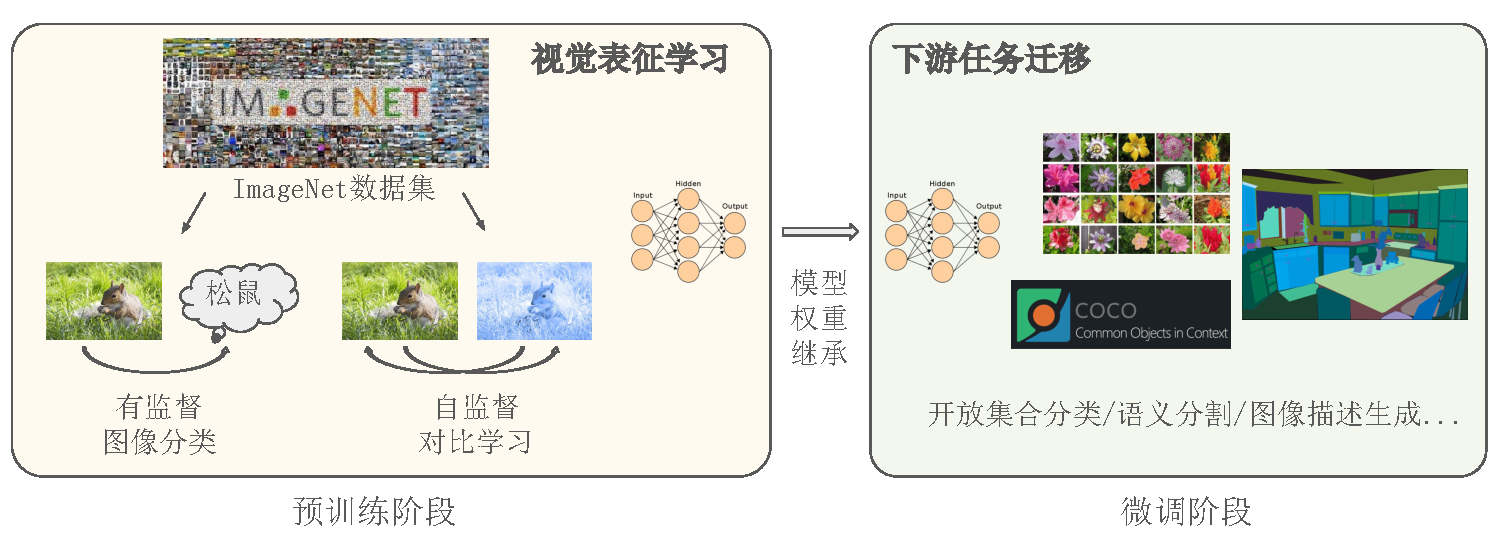
\includegraphics[width=1.0\linewidth]{figures/论文-图1-预训练-微调-v3.pdf}
  \caption{“预训练-微调”方法示意图}
  \label{fig:1-pt-ft-example}
\end{figure}

随着深度学习方法的发展,数据驱动已成为计算机视觉系统构建的重要范式。然而,获取大规模高质量的视觉任务标注数据需要耗费大量人力物力。为解决这一问题,研究者提出“预训练-微调”方法。通过将通用视觉表征学习与下游任务迁移过程解耦,“预训练-微调”方法有效缓解了任务数据收集难、标注贵的难题,提升了模型的性能表现。
% 如图\ref{fig:1-pt-ft-example}所示,预训练阶段通过大规模数据和代理任务驱动模型习得具有良好泛化能力的视觉表征,而微调阶段通过权重迁移实现模型对下游任务的适应。
“预训练-微调”方法如图\ref{fig:1-pt-ft-example}所示。在预训练阶段,模型基于ImageNet\cite{deng2009imagenet}等大规模基准数据集,通过有监督图像分类代理任务\cite{alexnet}或自监督对比学习代理任务\cite{chen2020simple}习得具有良好泛化能力的视觉表征。在微调阶段,通过模型权重继承和下游任务迁移方法,预训练模型在ADE20K语义分割\cite{zhou2019ade}、MSCOCO图像描述生成和目标检测\cite{chen2015microsoft}等视觉任务上进一步学习。
“预训练-微调”方法显著提升了视觉任务的数据使用效率和性能表现,已经成为计算机视觉领域的重要范式。
% “预训练-微调”范式将通用表征学习和任务能力培养拆分成两个阶段,显著提升了模型在各类下游任务上的数据利用效率和性能指标,缓解了下游任务数据收集难、标注贵的困境。
% “预训练-微调”范式促进了大语言模型和相关应用的发展与落地,但实现对物理世界通用感知的视觉模型研究进展仍较缓慢。人工智能领域的莫拉维克悖论\cite{mindchildren}阐明:“要让电脑如成人般地下棋是相对容易的,但是要让电脑有如一岁小孩般的感知和行动能力却是相当困难甚至是不可能的。”这一悖论也反映了视觉模型预训练研究的巨大挑战。% 需要从并列讲述视觉和语言过渡到视觉

% 0318,感觉还差一段描述视觉任务语义性的;但不知道加到哪里比较合适
% 视觉任务的本质是将像素级的图像信息映射到语义概念空间进行理解和推理。这一过程需要系统掌握从低层次的边缘、纹理特征到高层次的场景理解等多个层面的语义表达。由于视觉表征与语义概念之间存在显著的鸿沟,相同语义可能呈现出显著的视觉差异,而不同语义概念却可能具有相似的视觉表现。

% 难点-语义;标注依赖/跨任务泛化弱/细粒度建模不足
% 监督学习→封闭语义空间
% 自监督学习→无语义指引
% 共同缺陷→视觉单模态局限
% 解决方案→跨模态语言监督
视觉任务的核心挑战在于实现从底层像素级特征到高层语义级概念的有效映射。无论是图像分类、目标检测还是语义分割,都需要模型理解图像中物体和场景的语义内涵,并建立起视觉表征与抽象概念之间的关联。这种语义理解能力直接影响模型在开放环境下的泛化表现。
然而,当前主流的视觉预训练方法在语义理解层面仍有双重困境:基于图像分类的有监督预训练受限于封闭语义空间和稀疏标注信息,而基于图像自身的自监督预训练的视觉特征停留在感知层面,无法建立有效的语义理解能力。
具体而言,有监督图像分类方法通过人工标注的类别标签建立视觉感知到语义理解的映射,但其封闭式的类别空间导致模型语义覆盖范围狭窄,牺牲了模型在开放环境下的概念泛化表现,同时独热标签监督信号的语义稀疏性迫使模型建立粗粒度的图像-语义关联能力。此外,人工标注的数据成本限制了图像分类数据的大规模扩展。
% 此外,作为预训练代理任务,图像分类任务的监督信号较为稀疏,因此在预训练过程中容易出现模型过拟合现象,从而限制了模型习得表征的通用性。
% ImageNet分类预训练通过人工标注的类别标签建立视觉-语义映射,但其封闭式词汇表(1000-21K类别)导致语义覆盖狭窄。据JFT-300M研究显示,扩展至3亿标注图像仅能新增1.8%的细粒度概念,边际效益递减显著(Sun et al., 2017)。更严重的是,单热点标签(one-hot label)的监督信号存在语义稀疏性——ImageNet中每张图像仅关联1.05个语义概念(Deng et al., 2009),迫使模型建立粗粒度的类别决策面,牺牲了开放环境下的概念泛化能力。
自监督学习方法通过实例判别、掩码建模等基于图像内在结构的代理任务避免了对数据标注的依赖,但其学习目标局限于图像感知层面的空间连续性、平移不变性等统计特性,无法建立视觉表征与语义概念的关联。
% 这两种视觉预训练方法本质上都未能突破视觉单模态训练导致的模态孤岛效应,无法构建低层特征感知到高层开放语义理解的完整认知过程。
由于这两种视觉预训练方法本质上都局限于单一视觉模态的信息范围,因此难以构建从低层特征感知到高层开放语义理解的完整认知过程。
% 则可以大规模利用无标注的图像数据,避免了对数据标注的依赖,同时通过图像的空间连续性、平移不变性等特性驱动模型学习可泛化视觉表征,缓解了模型预训练过拟合的问题。然而,自监督预训练方法缺少对语义的建模,通过这种方法得到的模型无法理解语言信息。% 有点牵强的感觉。
% 自监督学习的语义失焦。虽然MoCo、BYOL等方法通过实例判别等代理任务突破标注依赖,但其学习目标局限于图像内在统计特性(如空间连续性、几何不变性)。实验表明,SimCLR在PASCAL VOC多标签分类任务中的平均查准率较监督预训练低14.7%(Chen et al., 2020),暴露其语义建模缺陷。这类方法构建的视觉表征缺乏与语言语义的系统性对齐,导致下游任务难以实现跨模态的知识迁移。
% 早期监督学习范式依赖ImageNet等标注数据集,通过图像分类任务学习语义映射。尽管该范式催生了ResNet等经典模型,但其标注依赖性和封闭类别空间导致表征的语义丰富性和迁移能力受限。随后的自监督学习(如MoCo、SimCLR)通过利用图像内在结构缓解标注依赖,但这类方法在高层语义建模上存在固有局限——旋转预测等代理任务难以建立视觉概念与开放语义的关联,导致模型在细粒度任务中出现语义失配。
% 这两种范式本质上都未能突破视觉单模态的语义隔离——监督学习受制于人工定义的封闭语义空间,自监督学习则困在无语义指引的特征空间。要构建开放语义的视觉智能,亟需引入语言模态的监督信号,通过跨模态对齐建立视觉概念与语言语义的动态连接。

% 曙光-自然语言
% NLP领域预训练模型的成功
% 大规模语言模型带来的启发
% 语言具有更丰富的语义信息+开放词汇
与此同时,自然语言处理领域研究通过大规模自监督预训练方法\cite{BERT,gpt2}在语义理解方面取得了突破性进展,推动了聊天机器人和智能体等应用的快速发展。相比视觉模态,语言模态具有天然的语义优势:它直接编码人类的认知概念,结构化表达能力强、语义泛化性优秀。语言模型在语义理解方面的成功,引发了研究者对视觉表征学习方法的思考:能否借鉴语言模态的优势来增强视觉表征的语义理解能力?
事实上,神经科学研究表明人脑在视觉信息和语言信息的获取和认知构建过程中展现出深层的协同机制\cite{bemis2013basic},例如角回脑区就同时参与了视觉场景解析和语义概念提取任务。这种认知层面的协同机制为利用语言模态作为视觉表征学习的语义先验提供了生物学依据。近年来,一些研究\cite{desai2021virtex,sariyildiz2020learning}已经探索了基于自然语言监督的视觉表征学习方法,并取得了初步进展。

% CLIP,引出需要前面更多过渡!
% 认知科学升维
%     引入fMRI神经影像证据强化理论创新性
%     通过t-SNE可视化建立方法可解释性
% 技术细节深化
%     明确模型架构细节(双塔/编码器类型)
%     量化关键实验指标(准确率/Recall@1)
%     列举典型应用框架(VIMA/DALL-E 2)
% 学术严谨性增强
%     补充图示引用(架构图/可视化图)
%     标注关键性能提升百分比
%     使用皮尔逊相关系数量化神经相似性
% 应用价值具象化
%     区分基础研究(认知模型)与应用领域(生成/具身/工业)
%     采用"方法论支撑"替代模糊的"促进发展"表述
% CLIP 通过“词的向量空间”和“视觉的向量空间”对齐,把视觉表征嵌入到语言所描述的概念中。
% 相比传统方法,它的优势在于:语义开放性(open vocabulary classification)+ 高效跨模态检索 + 强大的零样本能力。

语言-图像对比学习\cite{radford2021learning}(Contrastive Language-Image Pre-training,CLIP)方法作为基于自然语言监督的视觉表征学习里程碑方法,通过在混合图文数据中匹配正样本对实现跨模态表征对齐。这种方法将自监督对比学习思想扩展为多模态数据对比学习方法,在双塔架构中同步优化视觉模型\cite{dosovitskiy2020vit,resnet}与语言模型\cite{Transformer}来最大化配对图文样本的互信息,从而有效利用互联网中的大规模图文数据对构建感知与语义的统一表征空间。其中的代表性工作为OpenAI提出的CLIP工作\cite{radford2021learning}。
% ,通过多模态对比学习的思想,利用互联网规模的图文数据对进行预训练,实现了视觉表征与语言表征的对齐。这种方法有效利用了互联网中大量存在的图文数据对,解决了预训练数据可扩展性的问题。与此同时,该方法有效利用了文本信息对语义进行建模,赋予模型理解语言信息的能力。
% 通过语言-图像对比学习方法预训练得到的模型有效对齐了视觉表征和语言表征,使得相关表征间的距离更近,不相关表征间的距离更远。
通过语言监督信号,CLIP方法将图像分类任务中通过封闭类别空间表示的语义概念扩展至自然语言的开放词汇集合,在零样本开放集合图像识别任务上表现出色。通过可大规模扩展的互联网图文数据对,CLIP方法在视觉表征学习中注入了丰富语义先验,有效对齐了视觉表征与语言表征,可以高效实现零样本图文跨模态检索任务。
% 因此,这种模型无须微调,就可以被用于零样本图文跨模态检索任务中,同时也可以出色完成零样本开放集合图像识别任务,能有效增强搜索引擎的图文检索效果。
% 同时,通过语言-图像对比学习方法预训练得到的视觉模型具有更出色的语义信息理解能力,经过权重迁移到下游视觉任务时,增强了目标检测、语义分割等任务上的物体识别能力,从而进一步推动视觉模型研究的发展与进步。
语言-图像对比学习方法催生了一系列下游任务迁移研究:在图像生成领域,CLIP方法引导的扩散模型\cite{dall-e2}通过文本信息实现保真度高、准确性强的合成图像生成;在具身智能领域,CLIP方法作为多模态交互的认知基座\cite{llava},赋予了大语言模型视觉感知能力。
作为一种视觉-语言深度结合的预训练方法,CLIP方法已经成为“预训练-微调”范式中的重要一环,为构建通用人工智能的感知系统提供了关键支撑。
% 最近,研究发现语言-图像对比学习方法预训练的模型还可被用于基于文本的图像生成任务,同时也是赋予大语言模型视觉感知能力方法中的重要组成部分,促进了人工智能生成内容领域的繁荣。
% 因此,语言-图像对比学习方法因其可靠的数据可扩展性和对视觉信息与语言信息的有效建模能力,已经成为“预训练-微调”范式中的重要一环。


% 从领域发展过渡到实际科学研究,并提出pt-ft范式;
% 图一:左图预训练(需要上:图像)(下:文本)(左:有监督)(右:自监督);迁移;右图微调(上:图像)(下:文本)

% \todo{需要如何引出有监督和自监督,从而方便后文过渡到语言监督的视觉模型?}这里先不提,主要讲VL,可以较快引出CLIP,落回V之后再重提V的有监督等等

%%%
% 讨论联合微调的范式
% 主要引出解决多模态任务
%%%
% 总:近年来有相当多的工作考虑将两者当作已存在的独立模块,将其组装起来「使用联合微调」处理一系列VL的任务(这里可以扯一些应用,caption,grounding,qa等等),也就是说,他们使用各自领域的预训练,再将两部分模块组装「可以讲一下稍微现代点的VL-BERT系列?」;这种方案受限于原来各自预训练的好坏;
% 图二:可能是图一的延展,为了说明有联合微调,但是很少有联合预训练。注意需要迁移两部分权重。严格起见为了区分VL-BERT,可以把VL-BERT加入一个中间阶段,叫联合对齐?(预训练-对齐-微调)
% \begin{figure}
%   \centering
%   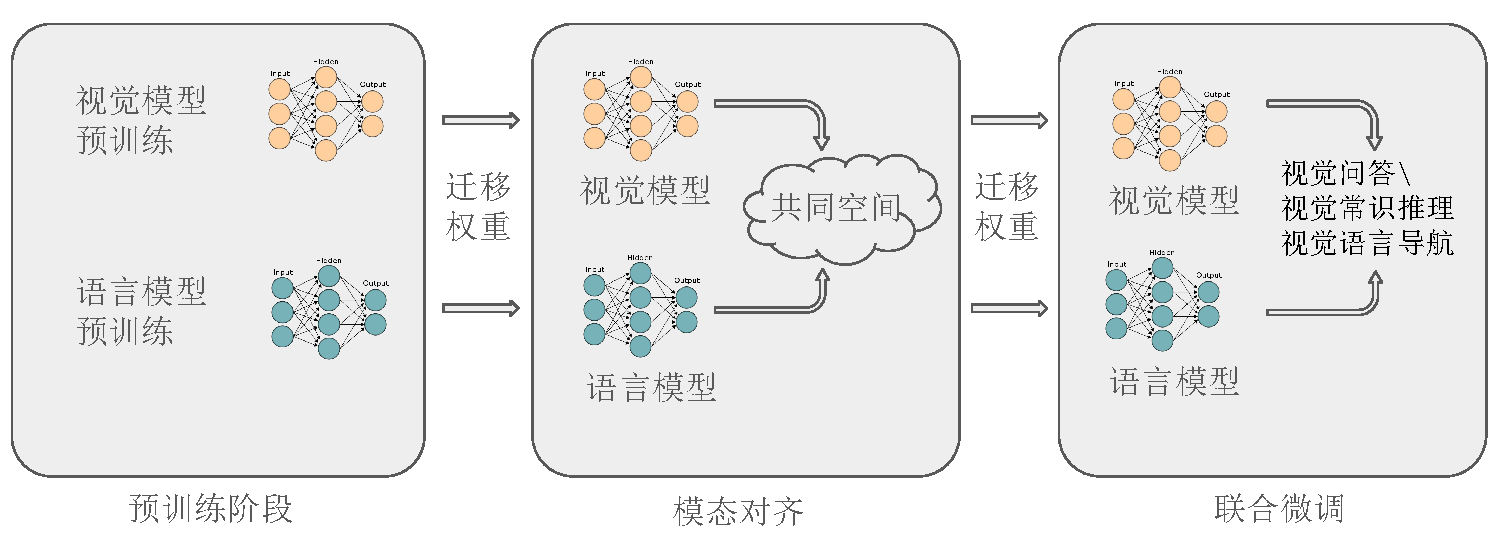
\includegraphics[width=1.0\linewidth]{figures/论文-图2-预训练-模态对齐-联合微调.pdf}
%   \caption{``预训练-模态对齐-联合微调''范式示意图}
%   \label{fig:2-pt-align-ft-example}
% \end{figure}
% 这种``预训练-微调''范式也被推广到了需要同时处理两种信息的多模态任务中,并出现了一种新的阶段:联合微调。如图\ref{fig:2-pt-align-ft-example}右侧所示,联合微调阶段是对微调阶段的扩展。该阶段分别继承预训练阶段得到的视觉和语言模型,在引入额外机制进行架构整合和信息融合后,在视觉问答、视觉常识推理、视觉语言导航等多模态任务数据上微调,以完成相应任务。
% 随着视觉-语言交叉领域的发展,研究者在``预训练-微调''范式中引入了一个中间阶段,称为模态对齐阶段。如图\ref{fig:2-pt-align-ft-example}中间所示,这一阶段是一种过渡阶段,其形式与预训练阶段类似,使用相对规模较大的多模态通用数据集对预训练阶段得到的单模态模型权重进行联合训练。这一阶段的主要目的是对齐语言的语义空间和视觉的感知空间,从而进一步提升模型在联合微调阶段的数据利用效率和性能指标。
% 联合微调阶段和模态对齐阶段的提出,促进了视觉-语言交叉领域的发展,催生了大量多模态场景和应用。

% 但是追本溯源,``预训练-微调''范式中的关键阶段在于预训练。因为微调阶段受限于数据标注成本高昂,获取难度大,无法扩大训练规模,而预训练阶段可以利用大量无标注或弱标注数据。
% 此外,微调阶段数据形式和目标相对确定,调整空间有限,而预训练阶段数据来源多样,代理任务设计更加灵活,提供了更大的提升空间。
% 同时,提升通用性是人工智能研究的长期追求。增强模型预训练阶段获得的能力,弱化微调阶段的重要性,是一个重要方向\cite{gpt3,gpt4}。
% 因此,越来越多的工作重点转向了预训练阶段的数据挖掘和方法设计。

%%%
% 视觉-语言的联合在认知学、心理学、脑科学等的支持,特别地引出具身智能学说
%%%

% 参考:具身假说:在大脑内部,思维是由负责视觉、行动和情感的同一套神经结构完成的,如果我们想要赋予语言意义,就要借助“感觉—运动”(sensory-motor)系统和情感系统,这些系统负责定义目标和想象、识别,以及付诸行动。进入21世纪后,越来越多的证据表明:心智与身体密不可分。。。。 具身革命业已证明,我们人性的本质、我们思考以及使用语言的能力,根本就是我们的身体与大脑合作的成果。人类心智的运作方式,从思想的本质到我们理解语言含义的方式,都与身体紧密相连,与我们在这个世界的觉察、感受与行动有关。我们不是冷血的思考机器,生理学为哲学提供了概念基础。
% 参考:具身模拟假说: 认为语言理解是人在心智中基于自己过去的视觉、听觉、运动等体验进行的模拟。具身模拟假说拥有大量认知科学、脑科学、语言学等学科的实验结果作为支持。。。人对语言的理解离不开身体与外界环境的互动,只有通过身体的视觉、听觉、运动等方面的经验积累才能实现对语言的理解,因此,有人认为脱离身体的语言理解是不可能实现的。在我看来:人工智能或自然语言处理的终极目标不应该是模仿人类,而应该是为人类提供有用的工具。从这个意义上来说,我们没有必要完全复制人类的语言理解过程,实际上,参考人类的处理机制,实现接近人类的语言处理能力应该就已足矣。
% 总:少有工作从源头上考虑两个模态共同预训练的可能。两者都有从互相模态信息中提取能力的可能(提一下之前BERT don't know how many legs of birds && Vision 一直使用受限Semantic Space的历史,泛化能力也会受label粒度影响(比如自然文本可以标蓝色衣服红色裤子小人,但是原来那种fix label set的只能标人,认识人但不认识腿之类))。

% ref: https://airs.cuhk.edu.cn/article/1124
% 随着人类对智能的理解进一步深入,越来越多观点认为智能是人类整个身体结构的综合表现,也即视觉的感知和语言的理解密不可分。研究者也提出了相关的具身假说\cite{understand, embodiment}。% Embodiment Hypothesis
% 具身假说认为,人类在大脑内部构建语言意义,是通过处理视觉、行动等功能的同一套神经结构完成的,也就是说,人类通过感知-运动-想象系统来理解语言意义。
% 进入21世纪后,有越来越多的脑科学、心理学和行为学的证据表明人的思维和感知密不可分,语言的意义无法脱离身体的感知进行构建,而语言又是表达感知、做出行动的重要方式。
% 无独有偶,在视觉预训练和语言预训练领域也都发现了类似的现象:缺乏语言引导的有监督视觉预训练方法通过无语义的类别分类作为代理任务,导致模型跨类别集合的泛化较为困难,限制了模型的迁移效果\cite{imagnettransfer};而纯语言预训练模型则可能在物理世界的常识问题上产生幻觉\cite{numersense}。

%%%
% 引出视觉-语言联合预训练的范式
% 落脚到视觉需要语言(怎么反驳不会语言的狗也有视觉能力!)
%%%
% 总:特别地,Vision model需要language才能对齐人类描述,所以Vision needs language more「这里要斟酌一下过渡,以及要不要提这也是本文的主要研究内容。」
% 参考:从演化认知的角度,这种跨模态协同机制可能源于早期人类的社会协作需求——当原始人类开始使用工具和构建居所时,必须通过语言符号将三维空间关系(视觉维度)转化为可传递的操作指令(语言维度)。这种进化压力促使大脑发展出独特的双通道处理架构:视觉系统负责建立实体世界的心理模拟,而语言系统则构建抽象符号的逻辑框架,二者通过前额叶皮层的高级调控实现动态耦合[6]。
% 图三:左图联合预训练(囊括模态对齐),右图分为三个部分(各自微调和联合微调);把各自微调加上是为了强调关注vision task!
% \begin{figure}
%   \centering
%   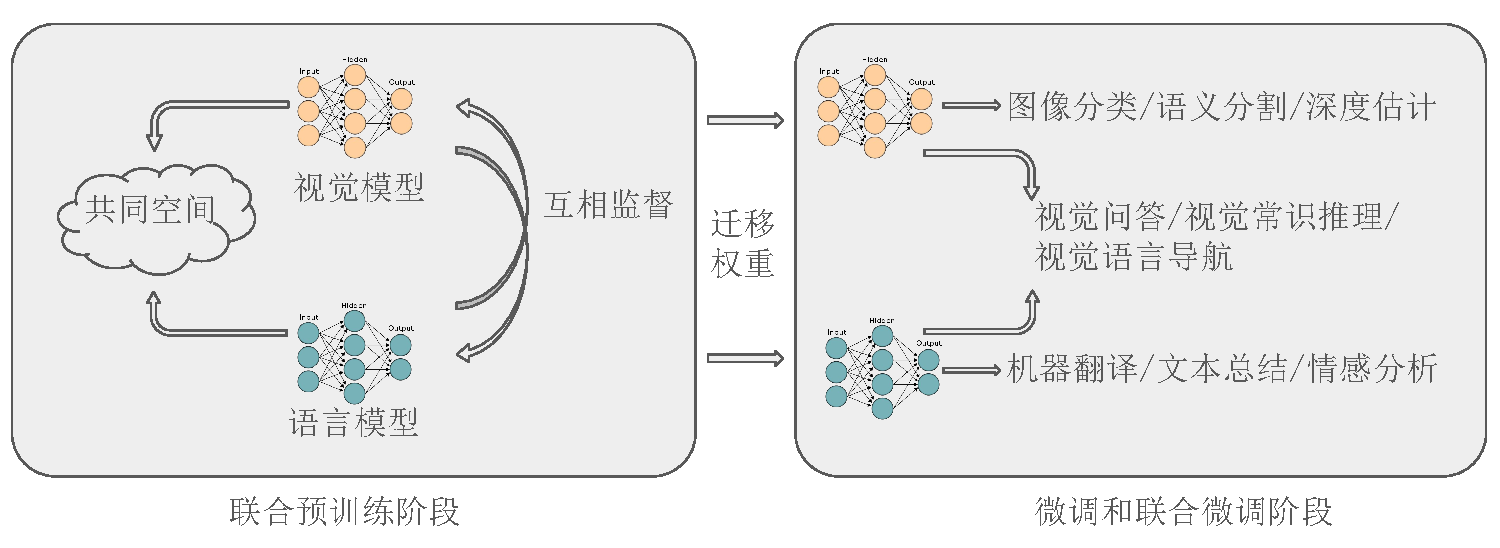
\includegraphics[width=1.0\linewidth]{figures/论文-图3-联合预训练-微调.pdf}
%   \caption{``联合预训练-微调''范式示意图}
%   \label{fig:3-fusept-ft-example}
% \end{figure}
% 认知神经科学的发现和人工神经网络的进展都展现了在预训练阶段同时处理视觉和语言信息,并从另一模态中学习的巨大潜力。在本文中,这一阶段被称为联合预训练阶段。
% 如图\ref{fig:3-fusept-ft-example}所示,这种方法将原本独立的视觉、语言预训练阶段合并,让视觉信息和语言信息互相监督,同时在预训练阶段完成原本模态对齐阶段的任务,无需引入额外的过渡环节,从而可以进一步统一和简化学习范式。
% Transformer\cite{Transformer}模型架构因其在图像信息建模\cite{dosovitskiy2020vit,Swin}与文本信息建模\cite{BERT,gpt2}任务上的出色表现,已经逐渐代替了原先有针对性设计的卷积神经网络和循环神经网络。Transformer网络从模型架构层面进一步统一了两种模态的处理方式。

% 但是长久以来,尚未找到足够高效,且有较强扩展性的“联合预训练”方法。
% 对人的生理、行为和智能理解支持了多模态“联合预训练”的出发点。这种方式从根本上从互相信息中学习,有更强的建模上限balabala。
% 视觉信息通过与语言系统的动态交互,形成了人类特有的符号表征能力。

% 回到从视觉模型的主体出发,因为CLIP本身就是这样的落脚点:Learning Transferable Visual Models From Natural Language Supervision
% 这里从联合收束避免讨论语言任务微调什么的还是比较重要的。
% 近年来大语言模型的成功\cite{gpt3,gpt4,palm,dsv3,chinchilla},以及视频生成模型在建模物理世界规律时遇到的挑战\cite{kang2024farvideogenerationworld},都在强调莫拉维克悖论(Moravec's Paradox)的正确性。
% 人类觉得更代表高级智能的数学、代码、写作等能力反而是当前人工智能领域进展较快的方向,而普遍认为对人类来说简单的任务,比如图像识别、运动理解、肢体行动等任务则进展缓慢。
% 这种发展速度的不一致性限制了当前人工智能系统的大规模应用。因此本文以视觉-语言联合预训练方法中的\textit{视觉模型}为主要关注点,进一步研究联合预训练的方法,并关注下游视觉任务和视觉-语言多模态任务的迁移效果,以期促进相关领域的进一步发展。

\section{语言-图像对比学习方法介绍及其研究目标}
本节主要介绍了CLIP方法的基本原理与研究目标。第\ref{sec:clip-introduce}节首先介绍了从早期基于人工标注数据的自然语言监督视觉表征学习方法,到借鉴视觉自监督对比学习思想的技术演进,并介绍了CLIP方法的具体实现方式,分析了CLIP方法在利用大规模互联网图文数据对方面的优势。第\ref{sec:clip-target}节分析了CLIP方法的两个主要研究目标:一是通过降低数据中语义噪声、扩展语义信息源来提升预训练视觉表征的语义理解能力,二是设计有效的迁移策略以增强模型在细粒度视觉任务和语义生成任务上的性能表现。

\subsection{语言-图像对比学习方法的发展与介绍}
\label{sec:clip-introduce}
% 先介绍一下语言-图像对比学习数据 % 可以画个这类数据的获取图
基于自然语言监督的视觉表征学习方法需要大规模的图文对训练数据。早期方法主要依赖众包平台(如亚马逊土耳其机器人\cite{AMT})收集人工标注的图像描述数据\cite{young2014flickr, chen2015microsoft}。这种方式虽然标注质量高,但数据收集成本昂贵、规模受限。CLIP方法另辟蹊径,转向利用网页中的图像替代文本(Alternative Text,Alt-Text)构建大规模训练数据\cite{YFCC100M, sharma-etal-2018-conceptual, changpinyo2021conceptual}。这些替代文本是网页代码中表述图像内容的文本属性,可以用于在图像无法显示时向视觉障碍用户传达图像内容,或供搜索引擎建立图文索引。因此这些替代文本天然包含了对图像内容的丰富语义描述。这种基于互联网的数据构造方式具有显著优势:数据收集成本低、来源丰富多样、语义覆盖广泛、且可以持续扩展数据规模。

% 早期基于自然语言监督的视觉表征学习方法过渡,为了进一步引出视觉对比学习方法
人工标注的高质量图像描述数据集\cite{young2014flickr, chen2015microsoft}促进了早期基于自然语言监督的视觉表征学习方法发展。基于这类数据的特点,这些方法主要借鉴了自然语言处理领域的成功经验。一类方法扩展了掩码语言模型\cite{BERT}的思想,通过要求模型利用图像信息预测被掩码的文本内容来学习视觉表征\cite{sariyildiz2020learning}。另一类方法借鉴生成式语言模型\cite{gpt2}的自回归设计,利用文本内容的马尔可夫性质,要求模型基于图像信息逐步生成完整的文本描述\cite{desai2021virtex}。这些方法强调数据中图像与文本之间的严格对应关系,要求文本准确、完整地描述图像内容。然而,这种严格的数据假设限制了这些方法在互联网图文数据对上的应用:网络数据中的文本描述往往包含噪声或不完整内容,且与图像的对应关系较为松散。这促使研究者思考一种更适合大规模、噪声化互联网图文数据对的视觉表征学习方法。

% 先介绍视觉模型自监督对比学习方法,为后续介绍CLIP方法提供铺垫
为了应对互联网图文数据对的噪声特性,语言-图像对比学习方法\cite{radford2021learning}借鉴了视觉自监督对比学习的核心思想。视觉自监督对比学习方法\cite{chen2020simple}基于图像的空间连续性、平移不变性等性质,对输入图像应用颜色变换、缩放裁剪、翻转旋转等数据增强策略,生成同一图像的不同视角。这种方法将来自同一原始图像的数据增强样本对定义为正样本对,将不同原始图像增强样本之间的配对定义为负样本对。通过最大化正样本对间视觉表征的相似度,同时最小化负样本对间表征的相似度,模型习得具有感知一致性的视觉表征。
% https://zhuanlan.zhihu.com/p/370782081
对比学习方法的关键优势在于它通过建模样本间的相对关系来学习表征。因此即使部分样本带有噪声,只要能保持相似样本的表征相对更接近、不相似样本的表征相对更远离这一基本相似度排序关系,模型就能学到区分性较好的有效表征。这种基于相对关系的学习策略提升了对比学习方法对数据噪声的容忍能力。

\begin{figure}
  \centering
  % \subcaptionbox{语言-图像对比学习方法概览\label{fig:6-CLIP-Method}}
  %   {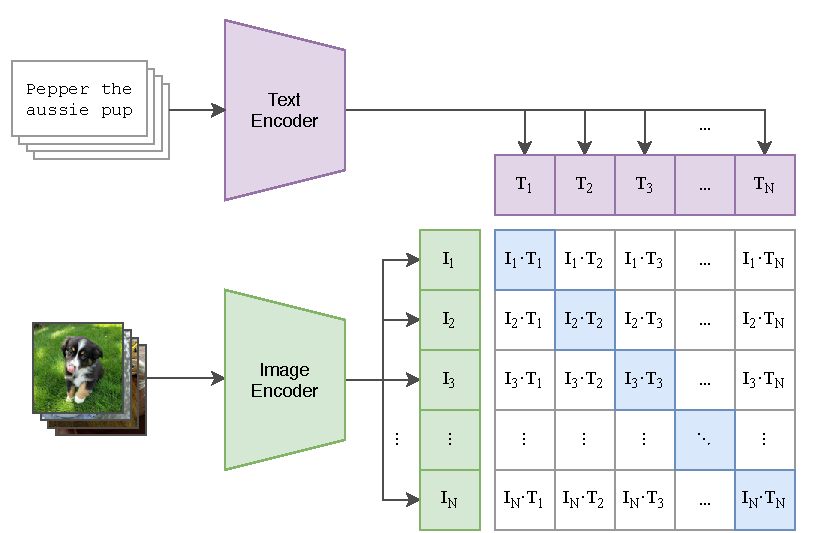
\includegraphics[width=0.48\linewidth]{figures/论文-图6-CLIP-方法.pdf}}
  % \subcaptionbox{语言-图像对比学习方法扩展性分析\label{fig:6-CLIP-Scaling}}
  %   {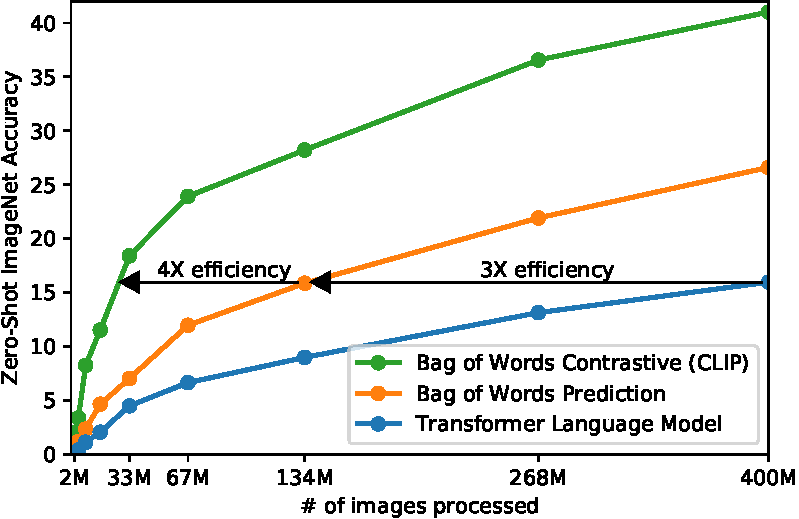
\includegraphics[width=0.48\linewidth]{figures/论文-图6-CLIP-效率.pdf}}
  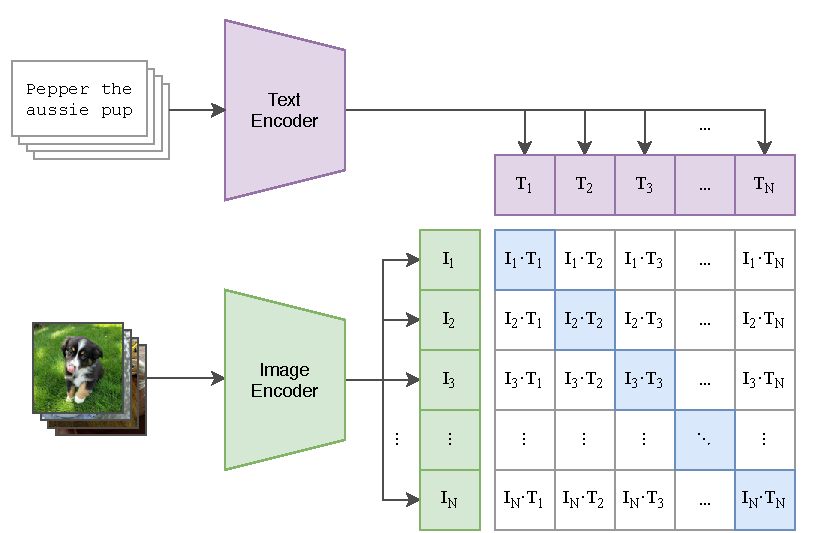
\includegraphics[width=0.9\linewidth]{figures/论文-图6-CLIP-方法.pdf}
  \caption{语言-图像对比学习方法\cite{radford2021learning}示意图}
  \label{fig:6-CLIP-Method}
\end{figure}

% 正式引出CLIP
% 互信息:https://www.bilibili.com/opus/776589765893947474 或者 https://zhuanlan.zhihu.com/p/583078368
% 通过最大化配对图文样本的互信息\cite{hjelm2018learning}
语言-图像对比学习方法创新性地将这种对比学习思想扩展到跨模态场景,从而有效利用带有噪声的大规模互联网图文数据对,并从中提取有效的语义信息进行视觉表征学习。
具体而言,CLIP方法将配对的图像和文本视作对同一物体或场景的不同模态描述以构建正样本对;而将不配对的图像和文本视作描述不同物体或场景的负样本对。与视觉自监督对比学习类似,CLIP方法在视觉表征与语言表征的共同空间中,拉近描述同一内容的跨模态表征,同时推远描述不同内容的跨模态表征。
如图\ref{fig:6-CLIP-Method}所示,给定一组$N$张图像$\mathcal{I}=\{I_1,\cdots,I_N\}$及其对应的文本$\mathcal{T}=\{T_1,\cdots,T_N\}$,CLIP方法的核心目标可以形式化为最小化如下比值:
\begin{equation}
    \min_{\theta}\frac{\sum_{i=1}^{N}f_{\theta}(I_i,T_i)}{\sum_{i\neq j;i,j\in[1,N]}f_{\theta}(I_i,T_j)},
    \label{eq:instance-level}
\end{equation}
其中$f_{\theta}$ 为距离度量函数。在实际实现中,CLIP方法构造了一个双塔架构,从而同时训练视觉模型$\theta_I$和语言模型$\theta_T$来提取两种模态表征,并采用InfoNCE对比损失函数\cite{oord2018representation}优化模型:
\begin{equation}
 \mathcal{L}_{I2T}=-\frac{1}{N} \sum_{i=1}^{N} \log \frac{\exp \left(\frac{\cos \left(\theta_I(I_{i}), \theta_T(T_{i})\right)}{\tau}\right)}{\sum_{j=1}^{N} \exp \left(\frac{\cos \left(\theta_I(I_{i}), \theta_T(T_{j})\right)}{\tau}\right)},
 \label{eq:infonce}
\end{equation}
其中$\cos(\cdot, \cdot)$表示表征间的余弦相似度,$\tau$为温度参数,用于调节正负样本对的对比强度。以文本为查询的对比损失$\mathcal{L}_{T2I}$形式类似,仅需交换图像与文本的位置。

从公式\eqref{eq:infonce}可以看出,CLIP方法通过优化图文样本对之间的相对距离来驱动学习。这种相对度量机制使得CLIP方法对图文对之间严格对应的数据要求较低。同时,通过温度参数$\tau$的调节,模型可以灵活控制表征对齐的程度。因此,CLIP方法相比于其他基于自然语言监督的视觉表征学习方法更适合处理互联网图文数据对:它不要求文本严格描述图像内容,而是通过对比学习框架来捕捉不同模态表达之间的语义关联,从而能够更好地利用大规模但带噪声的互联网图文数据对进行预训练。

% 语言-图像对比学习方法借鉴了这种思想,并将其推广到图文数据对中。具体而言,语言-图像对比学习方法将配对的图像信息与文本信息视作对同一物体或场景的不同描述视角,因此将它们称为正样本对,而将不配对的图像信息与文本信息视作描述了不同物体或场景的负样本对。
% 与实例级对比学习方法类似,语言-图像对比学习方法构建了一个图像表征与文本表征的共同空间,聚合描述同一物体的不同模态表征,分散描述不同物体的不同模态表征。
% 如图\ref{fig:6-CLIP-Method}所示,将一组$N$张图像记作$\mathcal{I}=\{I_1,\cdots,I_N\}$,将对应的一组$N$条文本记作$\mathcal{T}=\{T_1,\cdots,T_N\}$,并记模型参数为$\theta$,语言-图像对比学习方法可以被理解为最大化如下训练目标:
% \begin{equation}
%     % \max_{\theta}\sum_{i=1}^{N}\left[\log(f_{\theta}(I_i,T_i))-\sum_{j=1}^{N}\log(1-f_{\theta}(I_i,T_j))\right],
%     \min_{\theta}\frac{\sum_{i=1}^{N}f_{\theta}(I_i,T_i)}{\sum_{i\neq j;i,j\in[1,N]}f_{\theta}(I_i,T_j)},
%     \label{eq:instance-level}
% \end{equation}
% 其中$f_{\theta}$为距离度量函数。通常而言,语言-图像对比学习方法会同时训练一个视觉模型$\theta_I$和一个语言模型$\theta_T$来分别提取图像表征和文本表征,并用表征间的余弦距离作为距离度量方法。
% 因此在实际的训练过程中,语言-图像对比学习方法采用InfoNCE损失函数\cite{oord2018representation}驱动模型训练:
% \begin{equation}
%  \mathcal{L}_{I2T}=-\frac{1}{N} \sum_{i=1}^{N} \log \frac{\exp \left(\frac{\cos \left(\theta_I(I_{i}), \theta_T(T_{i})\right)}{\tau}\right)}{\sum_{j=1}^{N} \exp \left(\frac{\cos \left(\theta_I(I_{i}), \theta_T(T_{j})\right)}{\tau}\right)},
%  \label{eq:infonce}
% \end{equation}
% 其中$\cos(\cdot, \cdot)$表示图像表征与文本表征之间的余弦相似性。$\tau$表示温度超参数,控制了训练过程中正样本对与负样本对间的区别程度。式\eqref{eq:infonce}展示了语言-图像对比学习方法中以图像为中心与其他文本间的对比学习损失函数$\mathcal{L}_{I2T}$,而以文本为中心的对比学习损失函数$\mathcal{L}_{T2I}$则形式上与$\mathcal{L}_{I2T}$一致,只需要交换图像表征与文本表征的位置,这里不再赘述。

% 从式\eqref{eq:infonce}可以看出,语言-图像对比学习方法通过优化图文正样本对和负样本对间的相对距离驱动模型学习,并用温度超参数$\tau$来控制目标相对距离的幅度。这种方法对图像与文本信息一一对应的数据假设依赖较弱,并通过对比学习方式对齐了图像集合$\mathcal{I}$的表征空间和文本集合$\mathcal{T}$的表征空间。
% 因此,语言-图像对比学习方法更符合互联网中易收集的图文数据对的实际特性。相比于前述的视觉-语言多模态预训练方法,这种方法在扩展预训练数据时效率更高,可供学习的语义信息更为充足。

% 如图\ref{fig:6-CLIP-Scaling}所示,语言-图像对比学习方法\cite{radford2021learning}(绿色线)在ImageNet-1K数据集\cite{deng2009imagenet}零样本图像识别任务上相比于有监督图像分类方法(橙色线)有3倍的数据利用效率提升,而相比于从文本标注中学习视觉表征方法(蓝色线)则有11倍的数据利用效率提升。
% 天然提供了一项额外好处:\todo{简单的大规模检索算法和零样本开放集合识别} % 开放集合识别貌似基于回归的办法也可以做。可以提检索简化了识别(把open end的映射问题转为排序问题),对物体检测、语义分割都有帮助
% 因此,以语言-图像对比学习方法为核心的视觉-语言多模态预训练方法具备高效的数据利用能力和大规模数据扩展的潜力,同时通过对比学习的方式充分利用图文对中的语义信息,对齐了视觉表征与语言表征,已经成为重要的视觉-语言多模态预训练方法。

\subsection{语言-图像对比学习方法的研究目标}
\label{sec:clip-target}
% pt
作为一种新型视觉表征学习方法,CLIP方法利用大规模互联网图文数据对进行预训练,具有显著的数据可扩展性优势,但同时也面临着图文数据对质量参差不齐的挑战。CLIP方法尽管通过对比学习思想在一定程度上缓解了这个问题,放宽了文本严格描述图像内容的要求,但要提取有效的语义信息仍然需要保证图文对之间相似度的相对排序关系。因此CLIP方法的重要研究目标之一就是提升数据语义信号质量,增强视觉表征与语言表征的对齐效果。
% 此外,与传统视觉预训练方法相比,CLIP方法的核心创新在于借助语言模态强大的语义表达能力来指导视觉表征学习。
% 这种思路启发了进一步的思考:能否将计算机视觉领域积累的丰富标注资源转化为语言可建模的形式,作为对互联网图文数据对的有效补充?这些视觉标注涵盖了多个层次和不同描述角度的图像信息:从细粒度的物体标注(如目标检测的边界框、语义分割的像素类别、实例分割的物体轮廓),到中观层次的物体间关系(如空间位置关系、物体交互方式),再到宏观层面的场景语义理解(如场景类别、事件描述)。这些多层次、多维度的视觉标注信息为图像内容提供了丰富的语义描述。
% 将这些已有的结构化视觉标注转化为自然语言形式,不仅能为CLIP方法训练提供高质量的语义锚点,增强视觉表征与语言表征的对齐精度,还能扩展图像可用的语义信息来源,突破了CLIP方法对图文数据对形式的依赖限制。
此外,计算机视觉领域积累了丰富的有标注任务数据。这些视觉标注涵盖了多个层次和不同描述角度的图像信息:从细粒度的物体标注(如目标检测的边界框、语义分割的像素类别、实例分割的物体轮廓),到中观层次的物体间关系(如空间位置关系、物体交互方式),再到宏观层面的场景语义理解(如场景类别、事件描述)。这些多层次、多维度的视觉标注信息为图像内容提供了丰富的语义描述。
因此,这些数据为CLIP方法提供了高质量的准确语义锚点,增强视觉表征与语言表征对齐精度的同时,还扩展了图像可用的语义信息来源,突破CLIP方法对图文数据对形式的依赖限制。因此,在CLIP方法中有效引入已有的结构化视觉标注信息进行增强是CLIP方法的重要研究目标,也为整合现有视觉数据集提供了新思路。

% 作为一种视觉-语言多模态预训练方法,语言-图像对比学习方法的一个重要研究目标是如何扩展图文数据对、提高图文数据对质量,从而增强视觉表征与语言表征的对齐效果。
% 随着“预训练-微调”范式的发展,研究者总结出了一条重要的实践规律:扩展定律。针对语言模型中的扩展定律\cite{kaplan2020scaling, gpt4}研究显示,数据规模、模型参数量及两者共同决定的训练计算量是影响预训练方法效果及其在下游任务上迁移表现的重要因素,而数据质量差异和预训练算法设计则影响了扩展效率。扩展定律的提出直接促进了近期大规模语言模型的发展与应用\cite{gpt4,dsv3},而更多其他领域的“预训练-微调”范式研究\cite{henighan2020scaling, aghajanyan2023scaling, xie2023data}也进一步证明了扩展定律的有效性和可推广性。因此,增强语言-图像对比学习方法的预训练可扩展性,提高预训练扩展效率是此类方法的重要研究目标之一。

% ft
在提升预训练数据质量和语义覆盖范围的基础上,改进CLIP方法在下游任务上的迁移性能是另一个关键研究目标,也是“预训练-微调”范式的核心诉求。CLIP方法通过大规模图文数据对训练,实现了视觉表征和语言表征的对齐,因此在零样本图文跨模态检索和开放集合图像识别等直接利用跨模态表征对齐性质的任务上展现出优异表现。然而,视觉任务的多样性对预训练模型提出了更高要求:一方面,细粒度视觉任务(如目标检测、语义分割、深度估计等)需要模型具备密集预测和精细感知能力,而CLIP方法在实例级对比学习预训练过程中并未显式学习这些特性;另一方面,早期基于自然语言监督的视觉表征学习方法\cite{desai2021virtex}通过生成式训练,天然具备图像描述生成等语义生成任务能力,而基于对比学习的CLIP方法则缺乏这种能力。
因此,设计有效的迁移方法扩展CLIP方法应用范围也是CLIP方法的重要研究目标:首先,迁移方法需要充分利用CLIP方法强大的语义理解能力,同时增强其在细粒度视觉任务上迁移效果;其次,有效的迁移方法需要将CLIP方法的判别式视觉表征转化为生成式建模能力,使其能够实现更广泛的语义生成任务。这些研究不仅有助于提升CLIP方法的实用价值,也为探索通用视觉表征学习方法提供了新的思路。
% 在具备强可扩展性和高扩展效率基础上,如何提高语言-图像对比学习方法在各类下游任务上的迁移表现也是一个重要的研究目标。
% 前文提到,语言-图像对比学习方法利用图文数据对,对齐了图像表征与文本表征,因此在零样本图文跨模态检索和零样本开放集合图像识别等直接运用图像表征与文本表征对齐性质的任务上表现优异。
% 但是下游视觉任务类型多样,不仅包括ImageNet-1K数据集图像分类、iNaturalist数据集细粒度图像分类、MSCOCO图像描述生成等图像层面的语义理解或生成任务,也包括目标检测、语义分割、深度估计、光流提取等需要密集感知的细粒度视觉任务。
% 如何将语言-图像对比学习方法迁移到各类下游任务,同时广泛地提升其在各类下游任务上的性能表现同样是一项重要的研究目标。



% 视觉语言多模态预训练方法也经过了几个阶段的发展,早期以图像为条件的掩码语言模型比较流行。后来,它被从文本标注中学习视觉表征的方法逐渐替换,因为后者训练过程中的语义信号更加丰富。随着时代的发展,语言图像对比学习方法,也就是clip方法出现,因为这种方法的数据可扩展性更好,因此逐渐成为最重要的视觉-语言多模态预训练方法。

% 字符级联合预训练方法受自然语言处理领域的进展影响很大,其中两项代表工作分别是2020年提出的ICMLM\cite{sariyildiz2020learning}方法和2021年提出的VirTex\cite{desai2021virtex}方法。
% 两者分别是自然语言预训练方法中基于掩码语言词元建模模型BERT\cite{BERT}和基于语言自回归模型GPT\cite{gpt2}的拓展。其中基于自回归模型的VirTex方法(如图\ref{fig:5-character-instance}(a)所示)允许对自然语言监督信号进行充分利用,而ICMLM方法受限于掩码词元的比例不能过大,只能对监督信号的部分内容进行学习。
% 因此基于自回归模型的方法在下游任务上的迁移表现普遍优于基于掩码语言词元建模的方法。
% 这些小规模的研究工作首次证明基于视觉-语言联合预训练方法得到的视觉模型在图像分类、目标检测等下游视觉任务上可以取得良好的性能表现,同时无需额外的模态对齐阶段即可完成诸如图像注释(Image Captioning)等多模态任务,初步展示出视觉-语言多模态联合预训练方法的巨大潜力。

% 引出缺陷,引出CLIP,引出为什么CLIP好
% 达哥的缺陷是先讲了自监督的目标(迁移性好,扩展性强),然后讲实例级这两方面不好(迁移性特指dense tasks)他是先从实例级做起的,然而我上来就是CLIP)
% 随着研究深入,字符级语言监督的训练方法弊端逐渐显现,其中的核心原因是这种训练方法对图文配对数据的质量要求较高。这里将图片记作$I$,将长度为$n$的字符词元序列记作$T=\{t_1,\cdots ,t_n\}$,记模型参数为$\theta$,字符级语言监督方法本质上在最大化如下概率估计:
% \begin{equation}
%     \max_{\theta}\sum_{i=2}^{n}log\left({p_{\theta}(t_i|t_{1:i-1},I)}\right)    
%     = \max_{\theta}log\left({p_{\theta}(t_{2:n}|t_1,I)}\right)
%     \label{eq:character-level}
% \end{equation}

% 因此,此类方法强化了图文对的对应关系,其优化目标最终导向图像与文本的一一配对。
% 然而,这个假设在现实场景中很难成立。一方面文本描述千变万化,本身不存在强对应关系,另一方面这也与互联网数据的特性有关。
% 互联网中的替代文本与弱监督方法中的主题标题类似,虽然大部分是人类所写,但其质量良莠不齐,容易出现占位符、无关文本或低信息文本的情况,标注的信噪比较低。
% 因此,前述提到的两种字符级语言监督预训练方法均只在噪声比例较低的\{图像,文本\}对数据集,如MSCOCO\cite{chen2015microsoft}数据集上有成功应用,难以推广到以互联网替代文本为主的更大规模数据集\cite{sharma-etal-2018-conceptual}。
% 这一点限制了此类方法的可扩展性和方法上限。

\section{语言-图像对比学习方法的挑战与主要研究思路}
\label{sec:instance-challenge}

\subsection{增强预训练数据语义信号质量的挑战与研究思路}
% 缺陷一:数据噪声问题;前面从细粒度过渡过来的时候已经重提了噪声问题,怎么增强这部分的表述呢?泛化性好但是细粒度能力差(参考UniCL figure-6绘图)
预训练数据的规模和质量是影响模型效果的关键因素。互联网图文数据对中的大量噪声影响了CLIP方法视觉表征和语言表征的对齐效果。这些噪声主要来源于文本信息的低质量性和不规范性:作为图像的替代描述,网页中的替代文本往往由网页制作者随意编写,缺乏统一的规范要求和严格的质量控制。这导致了多种形式的数据噪声:一方面,不少替代文本与图像内容的语义关联性较低,如仅包含图像的文件名、网页链接或其他元数据信息;另一方面,部分替代文本可能完全不包含有效的语义信息,如重复字符、随机字符串等占位符文本。这些噪声数据不仅无法为视觉表征学习提供有效的语义监督信号,还可能误导模型建立错误的视觉-语言对应关系,降低预训练效果。更为根本的是,作为一种弱标注的数据来源,互联网图文数据对面临着质量提升与规模扩展的内在矛盾:强化语义质量控制往往意味着更高的获取成本,这将不可避免地限制数据规模的扩展。

针对这一问题,现有工作主要从降低数据噪声角度出发,提出了多种数据筛选策略:一类方法基于人工设计的规则(如文本长度、特殊符号比例、固定模式匹配等)进行筛选;另一类方法利用预训练好的小规模CLIP模型对数据质量进行打分;还有一些方法尝试利用ImageNet等图像分类数据集作为锚点,通过文本与类别匹配程度或图像相似度来筛选图文数据对。然而,这些方法都存在明显局限:基于人工规则的方法依赖专家先验知识,容易出现噪声遗漏或数据误删情况;基于CLIP模型打分的方法受限于对比学习的相对度量特性,难以提供可靠的绝对质量评估;基于图像分类数据的方法则受限于分类数据自身的封闭类别语义空间,限制了图文数据对的语义丰富度。
因此,如何设计有效的噪声控制策略,并探索新的可用语义信息来提升CLIP方法的视觉表征预训练效果,仍然是一个重要挑战。

基于上述挑战,本文提出了一个新的研究思路:进一步扩展CLIP方法借助语言模态强大的语义表达能力来指导视觉表征学习的核心思想,将其他形式的有标注图像数据转化为语言可建模形式,并通过对比学习框架实现多源数据的融合学习。具体而言,CLIP方法将配对的图像和文本视作同一内容的不同模态表达,通过对比学习实现视觉表征和语言表征对齐。这一思路可以推广到更广泛的数据形式:将任何配对的图像与其标注信息都视作同一语义概念的不同描述视角,从而将各类已有的视觉数据源统一使用对比学习框架建模。
这种方法具有双重优势:首先,现有的视觉标注数据通常经过严格的人工校验,具有较高的质量保证,因此将其整合到CLIP方法预训练过程中可以为模型提供准确的语义监督信号,提升预训练数据的整体质量;其次,不同类型的标注数据(如分类标签、场景类别等)从不同角度和粒度描述了图像内容,扩展了模型可获取语义信息来源的多样性。因此,该研究思路的关键在于选择合适的高质量标注数据,并设计有效的转化机制,使其能够融入CLIP方法对比学习训练框架。

% 因此,CLIP方法可以扩展到\{图像,文本,标注\}的三元组。
% 若进一步将标注转化为文本形式,这种\{图像,文本,标注\}三元组可以统一建模为\{图像,替代文本或标注文本\}的形式,使CLIP方法可以深度利用已有带标注的数据源进行训练。
% 考虑到已有数据标注往往经过不同程度的人工校对,且标注粒度有不同层次,信息覆盖角度多样,在一定程度上提升了整体数据的信噪比,因此这种方法对提升CLIP方法预训练过程中的数据效率也有一定帮助。
% mae/data2vec

\subsection{提升任务迁移性能和泛化性的挑战与研究思路}

% 缺陷二:迁移到下游视觉任务时,细粒度视觉任务表现不佳
CLIP方法通过实例级对比学习实现了视觉表征和语言表征的有效对齐,在图像识别、图文跨模态检索等全局语义理解任务上表现优异。然而,将CLIP方法的视觉模型迁移至目标检测、语义分割、深度估计等需要密集预测能力的细粒度下游视觉任务后,实验表明CLIP方法表现欠佳,无法充分利用其强大的语义理解能力。这一现象可以从CLIP方法的训练机制得到解释:如公式\eqref{eq:infonce}所示,CLIP方法中的视觉模型与语言模型通过池化操作或特殊标记分别提取图像和文本的全局表征进行对齐,忽略了图像局部信息与文本短语之间的复杂对应关系。这种对局部语义建模的缺失导致模型难以获得细粒度视觉任务所需的密集感知能力,但如何在CLIP方法中引入这种视觉任务是一个难点。

围绕这一问题,现有工作主要沿着两个方向展开:一类方法如局部化叙事\cite{LocNar}提出构建局部对齐图文数据对的高效标注方法,通过记录标注人员描述图像时的鼠标轨迹来建立文本片段与图像区域的对应关系。另一类方法如MaskCLIP\cite{MaskCLIP}则借鉴掩码图像模型\cite{he2022masked}思想,在CLIP方法训练过程中加入像素级图像重建任务。然而,前者方法需要昂贵的人工标注,难以规模化扩展数据;后者则需要设计复杂的多任务学习框架并重新预训练CLIP模型,计算成本较高。因此,如何以低成本方式增强CLIP方法的密集视觉感知能力,提升其在细粒度视觉任务上的迁移效果,仍是一个重要挑战。
% 主要研究思路。这部分内容zl其实没有,他写了缺陷,写了方法设计原则,但没有写方法思路。这部分zd写得比较多。
% 他们怎么都写了原则(zl)研究目标(zd),目前我还没写那么概括性的内容。

本文基于知识蒸馏\cite{hinton2015knowledge}的研究思路,提出了一个高效的迁移方法来应对上述挑战。虽然CLIP方法在训练过程仅进行了实例级对比学习,然而一些工作观察到其特征图中保留了一定的空间语义信息\cite{clipseg}。这种特征图级的视觉表征既包含了部分与文本对齐的语义知识,又保持了图像空间分辨率的特性。基于这一观察,本文提出通过特征图自蒸馏方式构建细粒度视觉训练目标进行迁移:使用预训练好的CLIP模型抽取视觉特征图作为蒸馏信号,指导新初始化模型训练。这种方法一方面通过有分辨率的特征图提供了密集预测能力所需的细粒度视觉训练信号;另一方面借助知识蒸馏机制高效地保留教师模型中蕴含的语义信息。相比现有方法,这种基于特征图自蒸馏的策略无需额外的数据标注,也避免了复杂的多任务学习框架,为增强CLIP方法在细粒度视觉任务上的迁移性能提供了一个简约且有效的方案。

% 缺陷三:如何迁移到下游视觉-语言交叉任务还不清楚
与此同时,CLIP方法得到的视觉表征与语言表征在判别式任务上表现优异。然而,与早期基于自然语言监督的视觉表征学习方法\cite{desai2021virtex}相比,CLIP方法缺乏直接的语义生成能力。这一局限源于两个方面:首先,对比学习框架主要强调表征的判别性,未显式训练生成式建模能力;其次,由于训练数据中的文本噪声较多,CLIP方法的语言模型在语言建模能力方面较弱,难以支持其迁移到图像描述生成、视觉问答等语义生成任务。

针对这一问题,现有工作尝试借助预训练好的大语言模型将CLIP方法的视觉表征转化为文本输出,来实现CLIP方法在语义生成任务上的迁移。然而,由于大语言模型仅在单模态文本数据上进行训练,其表征空间与CLIP方法的视觉表征间存在错位,因此需要通过整体微调重新建立两种模态表征的跨模态对齐。由于当前大语言模型通常包含数十亿甚至更多参数,这种微调策略的计算成本极其高昂。因此,如何设计更简单有效的迁移方法,使CLIP方法具有完成语义生成任务的能力,扩展其在更多下游任务上的应用,仍然是一个重要挑战。

% https://kexue.fm/archives/9119/comment-page-1
基于上述挑战,本文提出基于扩散模型实现CLIP方法在语义生成任务上的迁移方法。在图像生成领域中,扩散模型\cite{ddim,ddpm}因其强大的建模能力代替了生成对抗网络方法。而传统的语义生成任务迁移采用自回归方法\cite{gpt2},按从左到右的固定顺序依次生成文本内容。扩散模型通过迭代式的去噪过程实现生成式建模能力,相比于自回归方法具有独特优势:它允许模型同时利用前文和后文的信息进行建模,也支持对已生成内容的灵活修改,避免了自回归方法生成过程中的误差累积问题。然而,将扩散模型应用于语义生成任务迁移面临一个关键问题:不同于连续的图像信号,文本信号以离散标记形式存在。因此,该研究思路的关键在于为文本信号设计合理的噪声注入和去噪机制,构建有效的迭代去噪过程,从而实现CLIP方法在语义生成任务上的高效迁移。

% 最后,实例级视觉-语言多模态CLIP方法本质是一种对齐视觉表征和语言表征的预训练方法。CLIP方法将视觉表征和语言表征投射到一个共同空间,进而可以实现不同模态表征间的映射\cite{jia2021scaling}。
% 因此CLIP模型可以被视为一种视觉模态与语言模态互相转化的桥梁。Dall-E 2\cite{dall-e2}方法正是巧妙地利用了这种桥梁,利用扩散模型\cite{ddpm,ddim}将语言表征转化为视觉表征,进而完成基于文本的图像生成任务。这一思想同样可以被用于视觉表征向语言表征的转化,从而可以将CLIP模型迁移至一大类以文本为输出的视觉-语言多模态任务\cite{karpathy2015deep, vinyals2015show,vqa,vcr}。

\begin{figure}
  \centering
  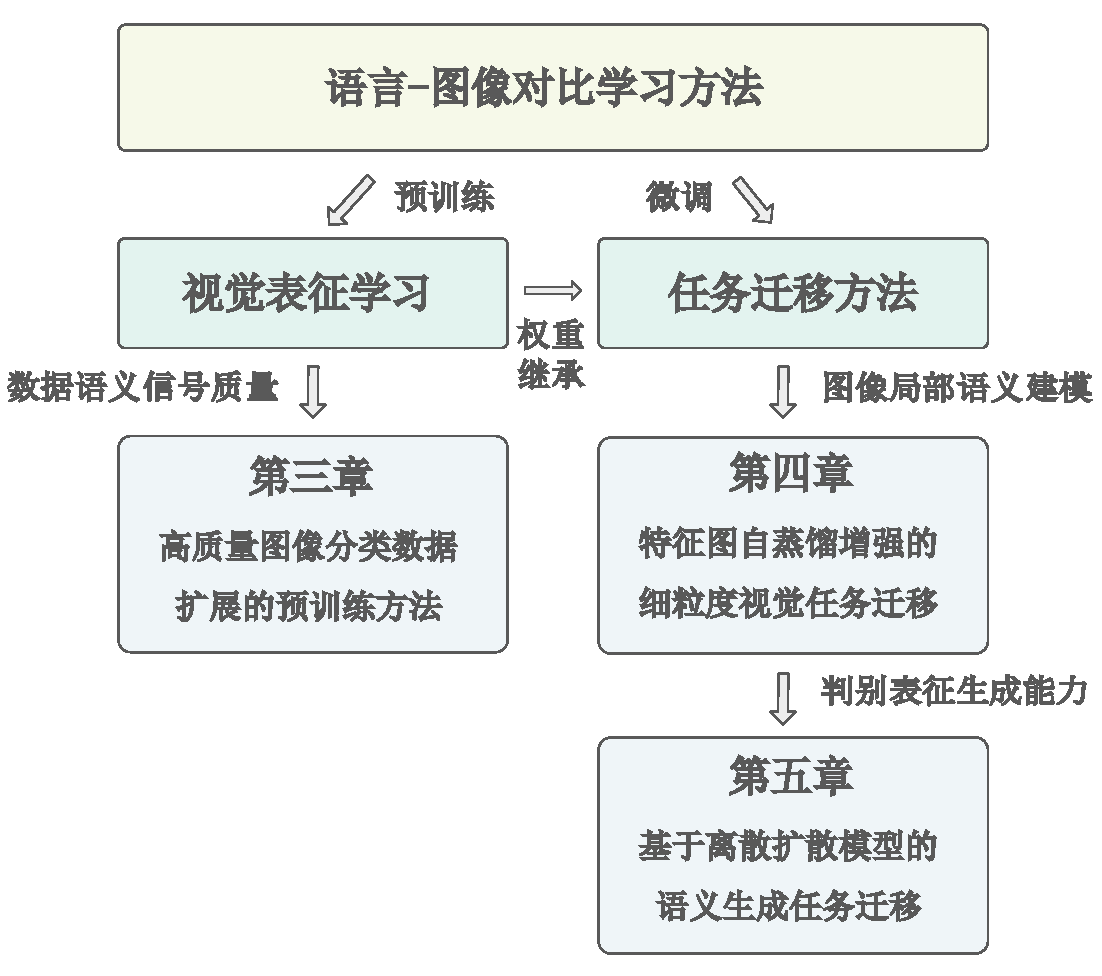
\includegraphics[width=0.9\linewidth]{figures/论文-结构安排-v3.pdf}
  \caption{本文的章节组织结构图}
  \label{fig:7-thesis-structure}
\end{figure}

\section{研究内容与主要贡献}
% 这两部分参考zl大哥的工作 1页
% 需要制作一个研究内容关系图,目标-挑战-思路-工作

如图\ref{fig:7-thesis-structure}所示,本文以语言-图像对比学习方法为核心,针对其在预训练数据语义信号质量和下游任务迁移性能与泛化性方面的关键挑战展开研究,提升了其视觉表征学习效果,增强了其在细粒度视觉任务与语义生成任务上的迁移表现。本文研究内容与主要贡献如下:

% 视觉表征学习和任务迁移方法
% 如何修改为楷体:https://www.cnblogs.com/LitBro/p/12074820.html
% 工作一:
\textit{提出基于高质量图像分类数据扩展的预训练方法。}
针对CLIP方法在预训练阶段面临的数据语义信号质量挑战,本文提出将对比学习框架扩展到更广泛的视觉标注形式,并重点研究了如何有效利用高质量的图像分类数据。具体而言,通过重新设计图像分类任务的损失函数和分类器类型,本文将图像类别标签从封闭语义空间中的序号转化为语言模态可建模形式,从而将图像分类任务纳入对比学习框架,进而提出了对图像分类数据与互联网图文数据对融合建模的iCLIP方法。为进一步丰富图像类别标签蕴含的语义信息,本文引入外部专家知识库作为补充,在对齐不同数据标注的语义粒度同时,增强了语言模型的语义建模能力。实验表明,新提出的iCLIP方法显著提升了视觉表征和语言表征的对齐效果,获得了语义信息更丰富的视觉表征,在零样本图文跨模态检索和开放集合图像识别任务上取得了明显性能提升。

% 工作二:
\textit{提出基于特征图自蒸馏增强的细粒度视觉任务迁移方法。}
% 视觉-语言多模态CLIP方法得到的视觉模型虽然蕴含了丰富的语义概念,并在对语义信息依赖较大的图像分类、图文检索任务上表现出色,但是它在一些弱语义的细粒度视觉任务的迁移表现并不惊艳,如物体检测、深度估计等任务。在这些任务上,CLIP的迁移表现与不依赖任何语义信息的自监督方法,尤其是像素级自监督预训练方法相比并无优势。
针对CLIP方法在依赖密集预测能力的视觉任务(如目标检测、语义分割、深度估计等)上迁移表现欠佳的问题,本文首先从输入完整性、训练目标粒度和损失函数设计三个维度分析了表现更优的像素级自监督方法,揭示了像素级训练目标对细粒度视觉任务迁移表现的关键作用。基于这一分析,本文提出利用知识蒸馏思想,将预训练好的CLIP模型输出特征图作为教师信号,指导新初始化学生模型训练。这种特征图自蒸馏方法一方面无需额外数据标注即可引入细粒度视觉训练目标,另一方面能够高效保留教师模型中的语义知识,避免重新预训练造成的训练成本。
实验表明,该方法仅需额外3\%的训练成本,就能显著提升CLIP方法在多个细粒度视觉任务上的迁移性能。通过对模型特征属性的诊断分析,本文发现自蒸馏后的CLIP模型具有与像素级自监督方法预训练模型相似的有效特性。更重要的是,特征图自蒸馏的迁移方法具有通用性:在含有三十亿参数的大规模视觉模型上应用特征图自蒸馏方法后,模型实现了目标检测和语义分割任务的性能突破,达到当时最优水平。

% 工作三:
\textit{提出基于离散扩散模型的语义生成任务迁移方法。} % 前面说很多方法用llm来做,比较昂贵,那这里是不就要提轻量?但我又没法和这样的模型去比较。我感觉我的工作的相关工作/context就是一坨。。时代发展确实有点快,2年没做就变天了。
CLIP方法虽然通过对比学习获得了判别能力强、对齐效果好的视觉表征和语言表征,但缺乏直接完成语义生成任务的能力。针对这一问题,本文提出了适配文本信号特性的离散扩散模型DDCap,从而实现CLIP方法在语义生成任务上的迁移。具体而言,针对文本的三个关键特性:离散性、低冗余性和序列长度可变性,DDCap方法设计了集中注意力掩码模块、长度预测任务和最佳优先推理策略,增强了CLIP方法在语义生成任务上的迁移效果。相比于传统的自回归方法,DDCap方法具有独特优势:一方面可以同时利用前文和后文信息,增强了对语义生成任务的建模能力;另一方面支持对已生成文本进行灵活修改,更适合人机交互场景。实验表明,基于离散扩散模型的DDCap方法在图像描述生成迁移任务上达到了与成熟自回归方法相当的性能水平,并在图像描述修改任务上表现更佳,验证了离散扩散模型作为语义生成任务迁移方法的巨大潜力。

% CLIP方法将视觉表征与语言表征映射到了一个共享的空间,搭建了模态之间互相转化的桥梁。一些前沿工作巧妙地利用了这一特性来完成基于文本的图像生成任务,但下游视觉-语言多模态任务中有一大类以文本为输出形式。如何利用CLIP模型解决这些基于图像的文本生成任务尚不清楚。
% 本文将针对图像生成领域主流的连续扩散模型推广为适配文本生成的离散扩散模型,首次探索了利用离散扩散模型实现基于CLIP方法的视觉模型进行文本生成任务的可行性。
% 相比于传统自回归方法,离散扩散模型允许模型同时查看前文和后文,增强了信息利用能力;并模仿了人类的写作习惯,允许对已经生成的文本进行修改,避免了自回归方法中前向误差累计的问题,更适合一些人机交互的场景。
% 本文方法从文本信号的离散性、低冗余性和变长特性三个方面入手,有针对性地设计训练方法和推理过程,并在图像注释生成这一典型任务上证明了CLIP方法的视觉模型与离散扩散模型组合的效果与潜力。

\section{论文的结构安排}
% 1页
% 每一章节讲了什么,需要绘图,可以把后面章节补起了之后加
% 本文的组织结构如图\ref{fig:7-thesis-structure}所示,共有6个章节。具体组织结构如下:

论文共分为6章,具体组织结构如下:

第\ref{cha:intro}章介绍了论文的研究课题——语言-图像对比学习方法的背景与意义,详细阐述了基于语言-图像对比学习方法在视觉表征学习和任务迁移方法两方面的研究目标、主要挑战和研究思路,最后总结了论文围绕语言-图像对比学习方法的研究内容与主要贡献。

第\ref{cha:relate}章回顾了传统视觉模型预训练方法,介绍了基于自然语言监督的视觉表征学习方法的发展历程,并讨论了语言-图像对比学习方法在增强视觉表征学习和扩展下游任务迁移方式两方面的研究现状。

第\ref{cha:iclip}章提出了基于高质量图像分类数据扩展的预训练方法iCLIP,首先分析了互联网图文数据对中的语义信号噪声问题,接着提出将对比学习框架扩展到图像分类数据后的多数据源统一建模方法,并引入外部专家知识库扩充图像类别标签语义信息,显著提高了CLIP方法在零样本开放集合图像识别和图文跨模态检索任务上的表现。

第\ref{cha:fd}章提出了基于特征图自蒸馏增强的细粒度视觉任务迁移方法,首先对比分析CLIP方法与像素级自监督方法的设计异同和迁移性能差异,接着提出特征图自蒸馏方法来引入像素级训练目标,无需依赖额外数据标注且大幅度保留预训练的语义信息,增强了CLIP方法在多个细粒度视觉任务上的迁移性能,并通过模型特征属性诊断工具分析了自蒸馏后的模型特性。此外,特征图自蒸馏方法还可用于提升其他预训练模型的迁移性能,验证了该方法的有效性和通用性。

第\ref{chap:ddcap}章提出了基于离散扩散模型的语义生成任务迁移方法DDCap,首先讨论了文本信号相比于图像信号的特殊性,接着提出适配语义生成任务的离散扩散模型迁移方法,讨论了集中注意力掩码模块、长度预测任务、最佳优先推理策略等训练方式和推理方式设计,接着利用该方法将CLIP方法迁移至图像描述生成和修改任务上,最后分析比较了DDCap方法与传统自回归方法的优劣。

第\ref{cha:summary}章总结了论文的主要研究成果,针对视觉表征学习和任务迁移方式两项研究目标讨论了现有工作的局限性,并探讨了增强CLIP方法的语义信号来源、提升下游任务迁移泛化性的未来研究方向。